\chapter{Análisis del problema \label{analisis}}
Este capítulo está dedicado a una explicación a fondo sobre el análisis del problema. Para ello se comentan los factores más relevantes sobre la fatiga muscular y su detección. Además se comenta un posible caso de lesión en rodillas a la hora de analizar la fatiga.


\section{Fatiga y sistema nervioso central}

La aparición de la fatiga durante la actividad física implica grandes cambios en la realización y percepción del esfuerzo. Esto hace que al realizar varias repeticiones, de por ejemplo en este caso, sentadillas, la acumulación de fatiga haga que cada vez realicemos una peor técnica y debido a esto aumenten las posibilidades de sufrir una lesión \cite{moreno2017fatiga}. Es decir, después de una sesión de entrenamiento, debido a la fatiga, no podemos realizar el mismo esfuerzo muscular y esto aumenta las deficiencias en la musculatura y puede llegar a provocar lesiones si no se trabaja con cuidado.


Otro factor a tener en cuenta, es que ciertos grupos musculares antagonistas pueden entrar en fatiga antes que otros debido a una mayor activación. Esto será tratado más a fondo en la sección de compensación muscular (Ver \ref{compM}). 

La fatiga está muy relacionada con el sistema nervioso central, ya que el sistema nervioso central (Ver \ref{fig:snc}) es el encargado de generar los impulsos eléctricos para que se produzcan las contracciones musculares. Cuanto mayor sean estos impulsos mayor grupo de motoneuronas serán implicadas y un mayor grupo de fibras musculares reclutadas, por lo que se tendrá una mayor fuerza física, así como un mayor control del peso cargado y una mayor técnica. Por ende si el sistema nervioso central está fatigado se tendrá un menor control del peso cargado, menor fuerza y peor técnica. Eso sería la llamada fatiga central, es decir, la fatiga del sistema nerviosos central.

Como bien se comenta en \cite{moreno2017fatiga} esta fatiga todavía es difícil de detectar, pero puede provocar una alteración en la transmisión del sistema nervioso central y en el reclutamiento de los axones motores. Debido a esto, el sujeto que está experimentando dicha fatiga no puede realizar toda la fuerza que sería capaz de realizar en condiciones normales, ya que como se ha explicado antes, no se reciben tantos impulsos para reclutar las fibras musculares. Esto hace que se vea reflejada una caída en la velocidad de ejecución de las sentadillas. Esto es debido a que la velocidad de ejecución y la fuerza realizada están muy relacionadas debido a que cuanto mayor es el número de fibras reclutadas mayor es la fuerza realizada y por consiguiente una mayor velocidad a la hora de realizar las sentadillas. Debido a esto, se ve bastante claro que fatiga y velocidad de ejecución en los entrenamientos son dos términos que están estrechamente relacionados.


\begin{figure}[ht]
\centering
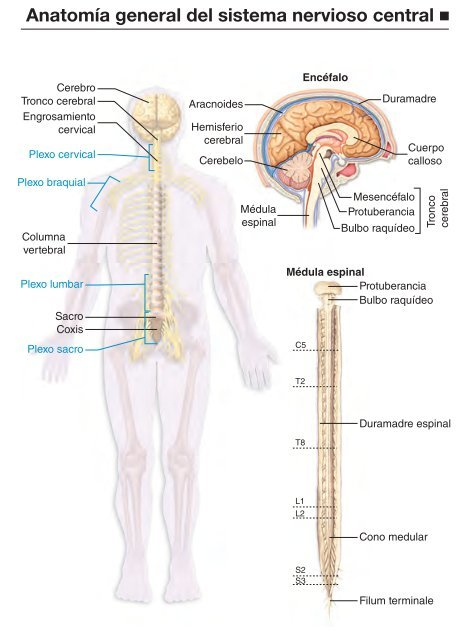
\includegraphics[scale=0.8]{imagenes/SNCcompleto.jpg}
\caption{Sistema nervioso central \cite{imagenSNC}}
\label{fig:snc}
\end{figure}


\newpage
\section{Velocidad de ejecución \label{velo condicion}}
Como bien se ha explicado anteriormente, la fatiga y la velocidad de ejecución son dos términos muy relacionados. Debido a ello un gran número de atletas actuales han basado sus entrenamientos en la velocidad de ejecución. Cuando detectan una caída de velocidad realizan un descanso de la actividad física, para no llegar a niveles muy extremos de fatiga y así poder sacar el máximo partido a sus sesiones de entrenamiento.

Para la detección de esta fatiga se ha estimado que la caída de velocidad de ejecución debe de ser de un 20 por ciento \cite{fernandezpropuesta}. Para ello se tendrá en cuenta dicho porcentaje con respecto a la primera repetición realizada.

A continuación se muestra una tabla-resumen, extraída de los datos utilizados para este proyecto, donde se pueden ver los valores de velocidad de ejecución de las 12 repeticiones registradas junto con el umbral de fatiga resultante. Finalmente una determinación de la fatiga muscular y una conclusión donde el entrenamiento debería de haber sido parado. Para la realización de este proyecto además de la caída del 20 por ciento en la velocidad, se ha estimado que dicha condición se debe de cumplir dos veces seguidas, es decir, en dos repeticiones realizadas consecutivamente, para así eliminar errores y obtener datos más precisos, ya que hay veces que existe caída de velocidad, pero no por fatiga, sino por factores externos, como la falta de concentración del atleta. 


\begin{figure}[ht]
\centering
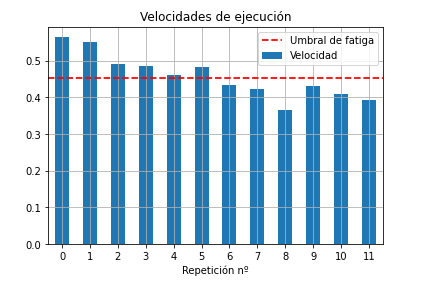
\includegraphics[scale=0.8]{imagenes/velocidades y fatiga.png}
\caption{Velocidad y umbral de fatiga}
\label{fig:fatiga}
\end{figure}

\section{Lesiones y compensación muscular}\label{compM}
Anteriormente se ha comentado que el hecho de realizar esfuerzo físico bajo una gran fatiga puede hacer que nuestros déficits, musculares o articulares aumenten, debido a la perdida de control del sistema nervioso central, y se produzca una lesión.

A parte de esto, en sujetos que ya tienen una lesión en la rodilla, esto se ve más incrementado. Por ejemplo en la lesiones de ligamento cruzado anterior (Ver \ref{fig:lca}), se ha detectado que las personas que la sufren experimentan una serie de cambios en la musculatura de su pierna. En este estudio realizado sobre personas con dicha lesión \cite{kim2018influencia} se demuestra que existe cierta compensación muscular entre los cuádriceps y los isquiotibiales cuando se sufre dicha lesión. Se demuestra que al haber sufrido una rotura del ligamento cruzado anterior, se produce un perdida de fuerza en la musculatura implicada en la rodilla, isquitibiales y cuadriceps. Sin embargo, esta perdida de fuerza es mucho mayor en los cuadriceps que en los isquiotibiales. Esto es  debido a que los pacientes con el ligamento cruzado anterior lesionado, producen una compensación muscular. Se debe a que los cuadriceps son los encargados de la extensión de la rodilla y los isquiotibilaes de la contracción de esta. Por ello, cuando existe dicha lesión, el isquiotibial no deja que el cuadriceps funcione a plenitud, para así, evitar una fuerte extensión de rodilla y evitar producir una gran tensión en el ligamento anterior cruzado, el cual, está dañado.

\begin{figure}[ht]
\centering
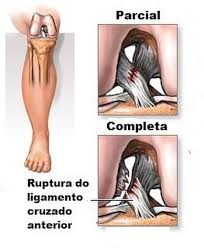
\includegraphics[scale=0.75]{imagenes/lca.jpeg}
\caption{Ligamento cruzado anterior: lesión parcial y completa \cite{imagenLCA}}
\label{fig:lca}
\end{figure}


Para ello la detección de la fatiga mediante diferentes clasificadores que reciban la información de los diferentes músculos examinados, puede ser clave para ver que músculos entran antes en fatiga, y si se produce en el orden correcto. Si no es así, sería un gran indicativo de que existe cierta anomalía en la rodilla. 

Por ejemplo, en la ejecución de una sentadilla, la activación de los cruadriceps debería de ser siempre mucho mayor que la de los isquiotibiales.





